\documentclass[journal,onecolumn]{IEEEtran}

% include a few useful packages; you will probably want more
\usepackage{graphicx} 
\usepackage[margin=1in]{geometry} 
\usepackage{amsmath,amsthm,amssymb}
\usepackage[noend]{algpseudocode}
\usepackage[hypcap=true]{caption}
\usepackage{lipsum}
\usepackage{float}
\makeatletter
\def\BState{\State\hskip-\ALG@thistlm}
\makeatother
\usepackage{algorithm}
% place all photos and diagrams in the media folder
\graphicspath{{media/}}

\hyphenation{op-tical net-works semi-conduc-tor}

\begin{document}

\title{%
  ROB 550 BotLab Report \\
  %\large Prototype Implementations of SLAM and A* for a Wheeled Robot
  }
    
\author{Saptadeep Debnath - saptadeb@umich.edu}

\maketitle

\IEEEpeerreviewmaketitle

\section{MAPPING AND SLAM}

\subsection*{1.1 - Mapping - Occupancy Grid} 

The mapping function is implemented in two stages. First we score the cells which are located at the endpoint of the rays. If the cells corresponding to the endpoint of the rays are in the given map, log odds for the cell are increased by `3', defining the boundaries. Next, the cells between the robot cell and the endpoint cell are scored by raterizing the given ray using the Bresenham's line algorithm. The log odds of these free cells are then decreased by `1'. 

The maps generated when the robot is stationary as is in the case of convex\_grid\_10mx10m\_5cm.log are not quite accurate at far away points. When the robot is stationary the laser rays originating from that position diverge farther away from each other at long distances, because of which some of the cells in between those rays don't get scored. This problem is mitigated when the robot is in motion; wherein because of the motion of the robot the laser rays tend to cover most of the grid cells and hence we obtain a better map in the end.  

\subsection*{1.2.1 - MCL - Action Model} 

Out of the two most widely used motion models, odometry motion model is used over the velocity motion model for this project. Odometry information is obtained by integrating the wheel encoder information over periodic time intervals. It is however observed that even though the odometry action model isn't perfect, it provides a better approximation of the robot motion than the velocity model for predicting the robot motion.

In order to predict the robot pose the odometry information (i.e. x, y and $\theta$) is changed to an RTR information given by equation \ref{eq:RTR}, i.e rotation-translate-rotation which is sampled with a Gaussian noise distribution in the form described in equation \ref{eq:fullRTR}. In the initial phases of the project the values of the noise constants were chosen as $k_1 = 0.8$ and $k_2 = 0.3$. On further inspection and to reduce the computation load to calculate the standard deviation for each odometry information, the standard deviations are given as constants, where ${\sigma}^2_{rot1} = 0.05$, ${\sigma}^2_{trans} = 0.005$ and ${\sigma}^2_{rot2} = 0.05$. These noise constants are chosen and tuned in order to achieve a better spread of distribution of the particles and to achieve a more accurate proposal which is used for the sensor model. It is expected to see the tuning parameters differ from one mbot to another, but the difference should be small as the make and model of the mbot is consistent The elements which could factor into a possible drastic difference between the tuning parameters from one mbot to another could be the systematic errors related to the specific mbot. It is observed from the following figures that after each run the particles are hugely spread over the map, which in turn is quite useful for a action model, as it is able to cover a large area for the robot pose distribution which can be further corrected by the sensor model. 

\begin{equation}\label{eq:RTR}
\begin{split}
	\delta_{rot1} &= atan2(y_t - y_{t-1}, x_t - x_{t-1}) - \theta_{t-1}	\\
	\delta_{trans} &= \sqrt{(x_t - x_{t-1})^2 - 	(y_t - y_{t-1})^2}	\\
	\delta_{rot2} &= \theta_t - \theta_{t-1} - \delta_{rot1}
\end{split}
\end{equation}

\begin{equation}\label{eq:fullRTR}
\begin{split}
	\hat{\delta}_{rot1} & \sim \mathcal{N}(\delta_{rot1},\,k_1 \cdot \mid\delta_{rot1}\mid)	\\
	\hat{\delta}_{trans} &\sim \mathcal{N}(\delta_{trans},\,k_2 \cdot \mid\delta_{trans}\mid)	\\
	\hat{\delta}_{rot2} &\sim \mathcal{N}(\delta_{rot2},\,k_1 \cdot \mid\delta_{rot2}\mid)
\end{split}
\end{equation}

\begin{figure}[H]
\centering
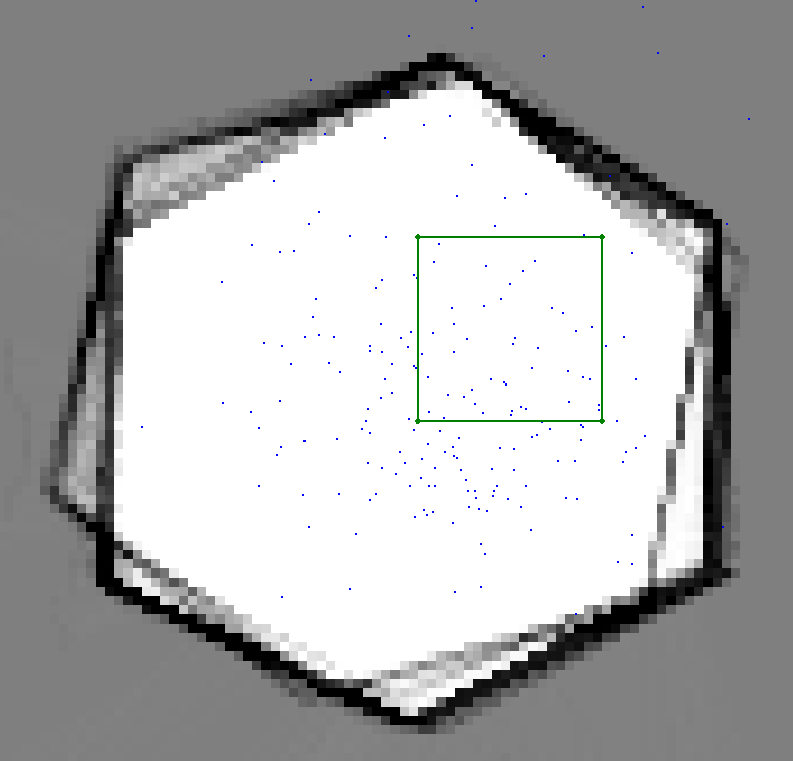
\includegraphics[width=0.3\textwidth]{Media/1211.png}
\caption{Particle distribution obtained at the end of drive square with action only}
\end{figure}

\begin{figure}[H]
\centering
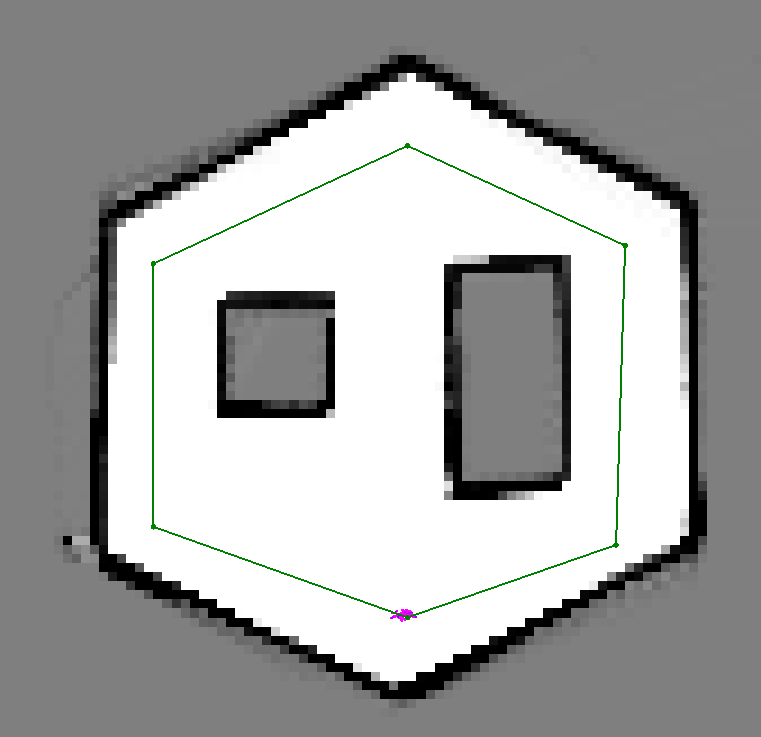
\includegraphics[width=0.3\textwidth]{Media/1212.png}
\caption{Particle distribution obtained at the end of obstacle slam with action only}
\end{figure}

\begin{figure}[H]
\centering
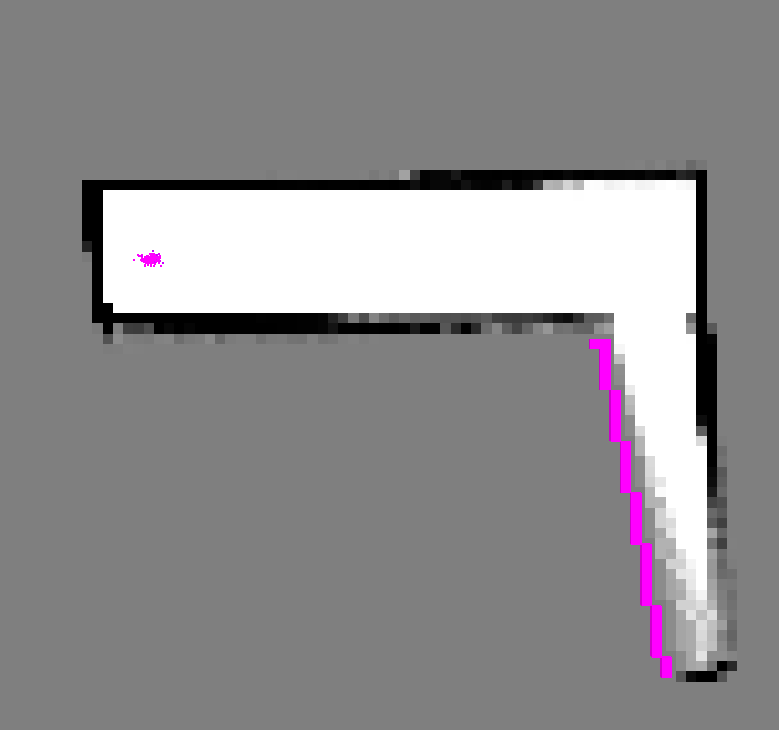
\includegraphics[width=0.3\textwidth]{Media/1213.png}
\caption{Particle distribution obtained at the end of straight line calm with action only}
\end{figure}

\subsection*{1.2.2 - MCL - Sensor Model \& Particle Filter} 

A simplified likelihood field model is implemented which overcomes the lack of smoothness and computational limitations of the sensor beam model. The sensor model function scores a given ray, by inspecting the endpoints of the ray. If the endpoints of the ray are occupied, i.e. is the cell at the endpoint of the ray is an obstacle, the log odds of that cell is returned. But in case the endpoint is not an obstacle, the ray is extrapolated in the forward and backward direction by one cell and a fraction (0.5) of their log odds is added to the score. These ray scores are then used as weights for a given particle. Since, the sensor model acts as a correction step, the pose estimate is almost similar to the true pose. It is observed that the sensor model performs well and the particles tend to remain in a tight region as the robot moves. The particles though have a tendency to spread if the robot rotates aggressively, but the come closer as the robot starts to move again.


\begin{figure}[H]
\centering
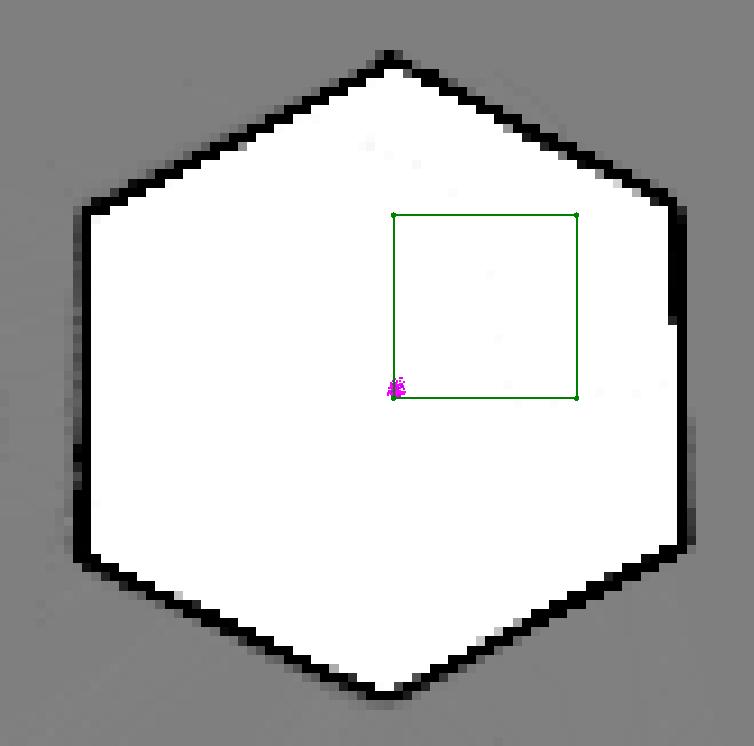
\includegraphics[width=0.3\textwidth]{Media/1221.png}
\caption{Particle distribution obtained at the end of drive square with localization only}
\end{figure}

\begin{figure}[H]
\centering
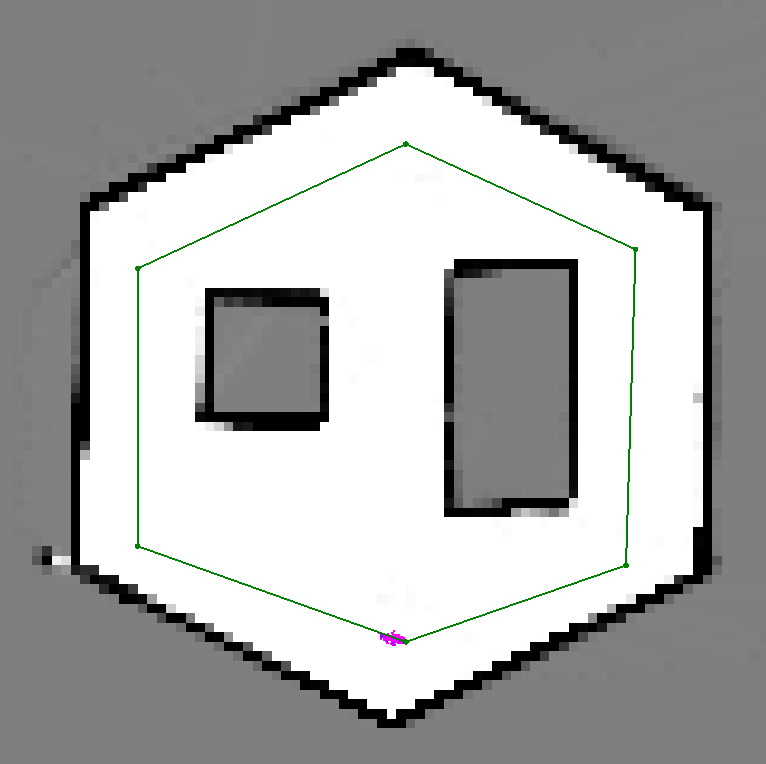
\includegraphics[width=0.3\textwidth]{Media/1222.png}
\caption{Particle distribution obtained at the end of obstacle slam with localization only}
\end{figure}


\begin{figure}[H]
\centering
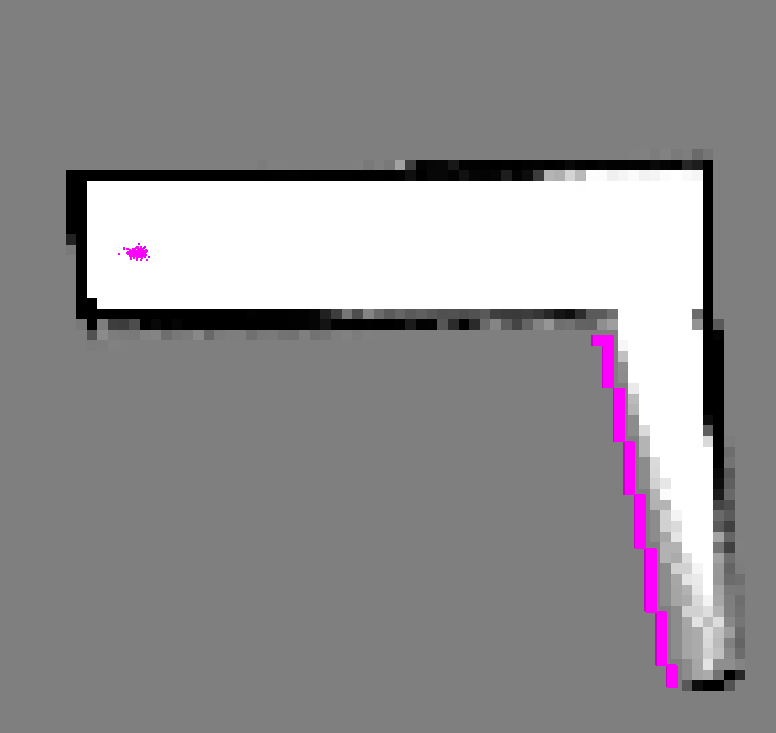
\includegraphics[width=0.3\textwidth]{Media/1223.png}
\caption{Particle distribution obtained at the end of straight line with localization only}
\end{figure}

\subsection*{1.3 - Simultaneous Localization and Mapping (SLAM)} 

In the previous two runs, the slam code is implemented by providing the already generated map of the environment to the system, for it to localize the robot either just by providing a proposal using the action model, or by providing the posterior of the robot pose by using the sensor model to correct the robot pose. But in the case of running the full slam code, the function simultaneously maps the environment and localizes itself in the generated map. Since, the map is generated simultaneously, it is expected to have a higher computation time compared to the previous two runs. But it is observed that the performance is quite close, which is due of the optimal mapping algorithm which generates the map without using much computation power. 

The change in map resolution from 5cm grids to 2cm grids seem to increase the computation time, but it doesn't effect the slam results that much. Although because of the smaller grid size the resultant maps generated are much smoother as compared to the previous maps.


\begin{figure}[H]
\centering
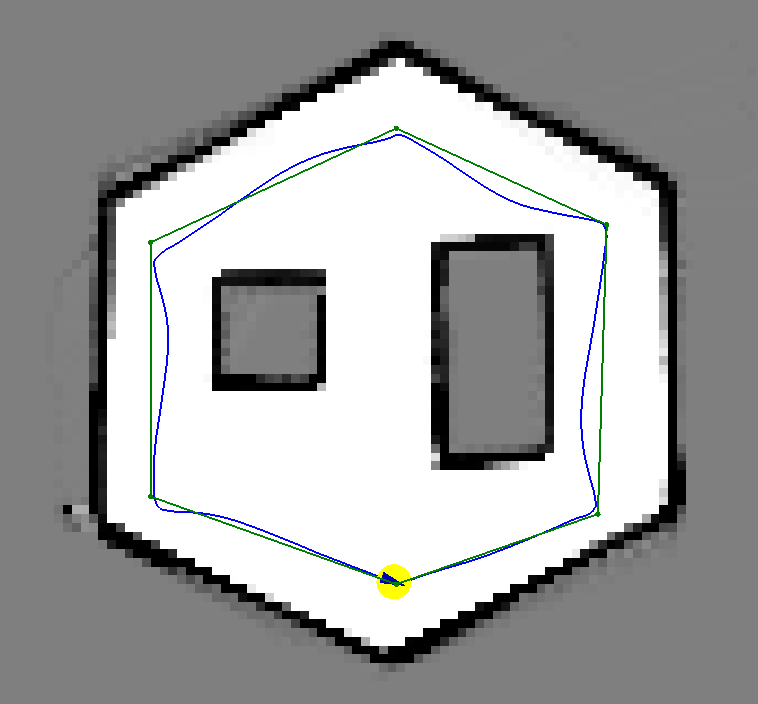
\includegraphics[width=0.3\textwidth]{Media/131.png}
\caption{Particle distribution obtained at the end of Obstacle Slam with Full SLAM}
\end{figure}

\begin{figure}[H]
\centering
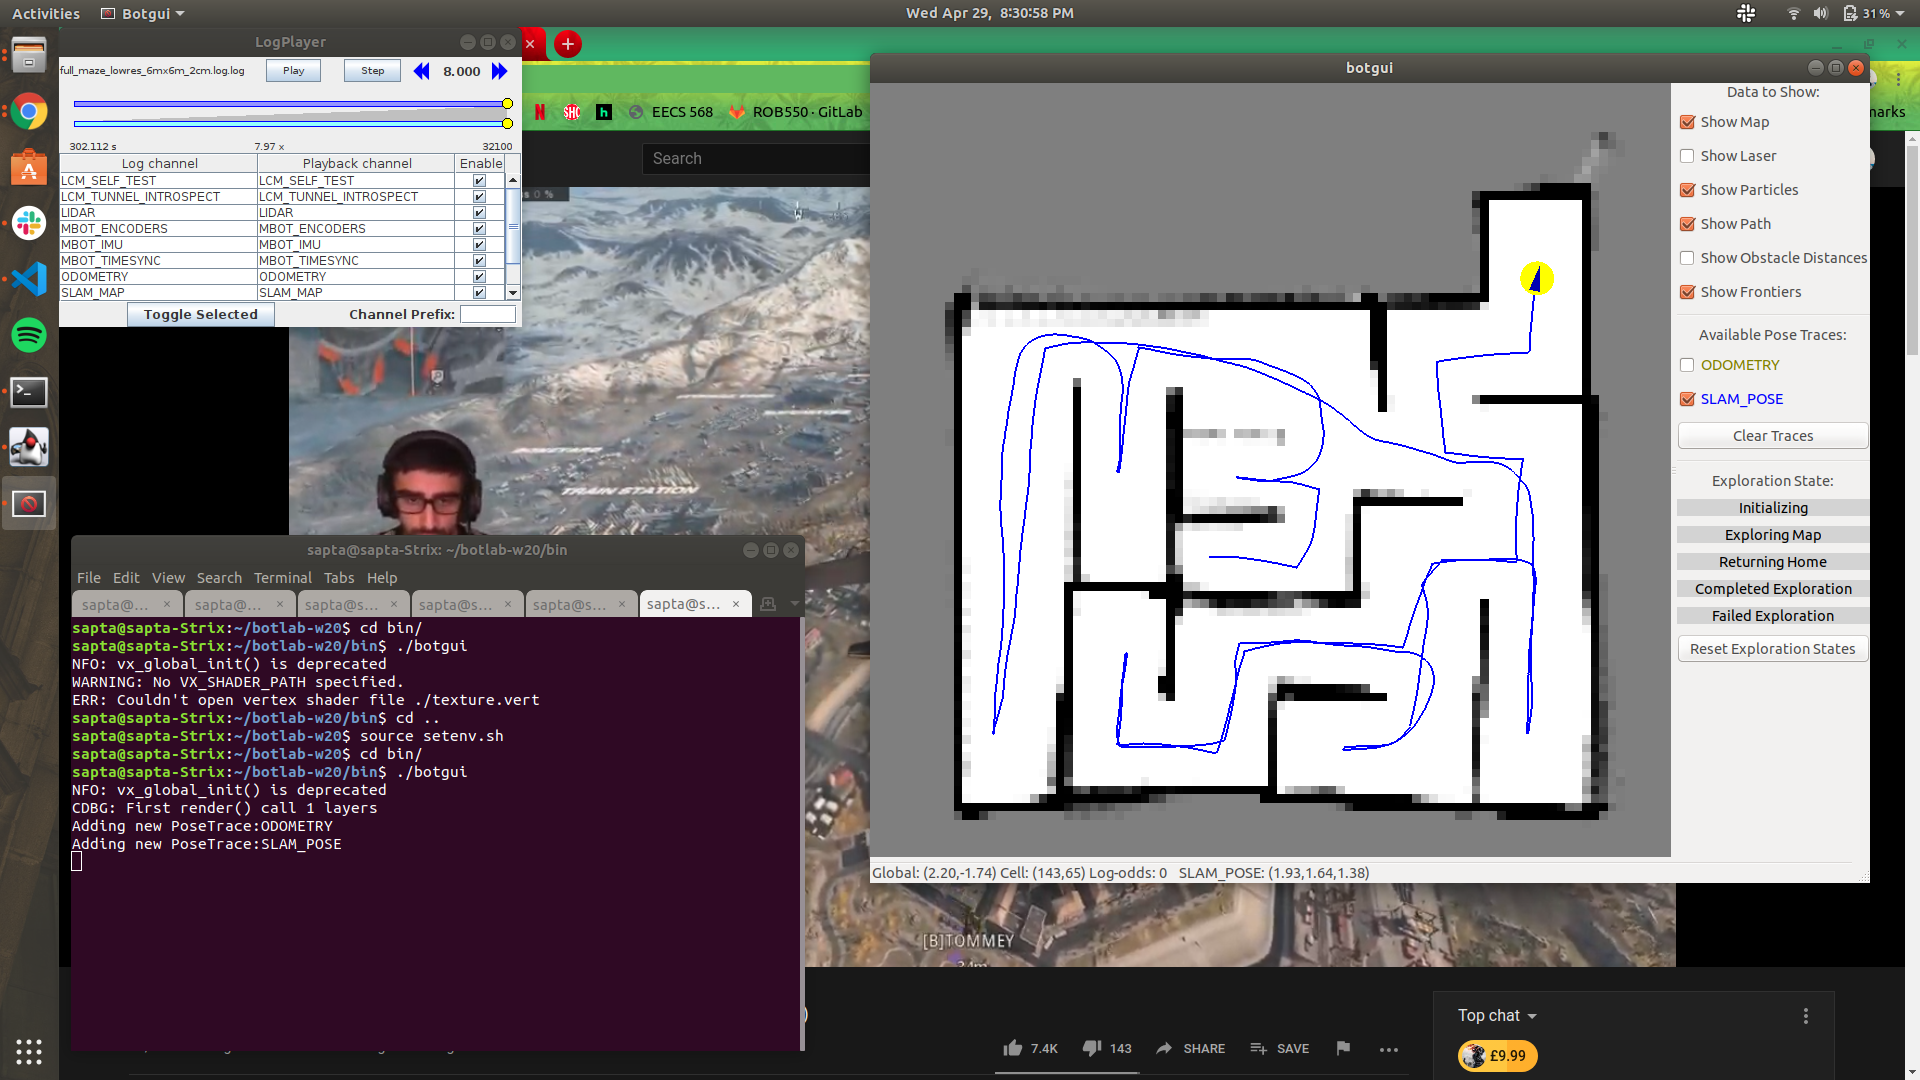
\includegraphics[width=0.3\textwidth]{Media/132.png}
\caption{Particle distribution obtained at the end of Maze LowRes with Full SLAM}
\end{figure}

\begin{figure}[H]
\centering
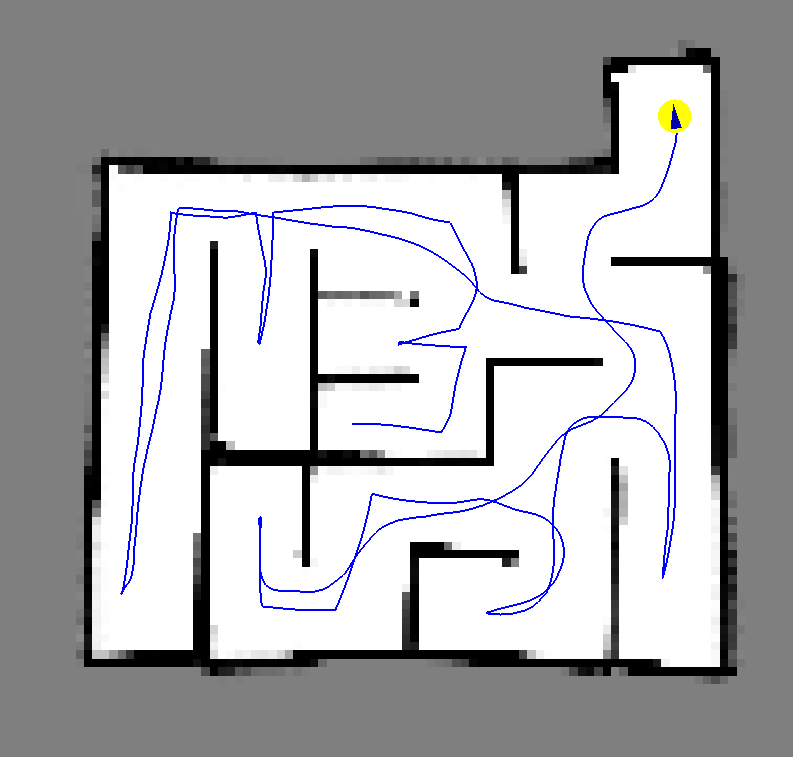
\includegraphics[width=0.3\textwidth]{Media/133.png}
\caption{Particle distribution obtained at the end of Maze HiRes with Full SLAM}
\end{figure}

\begin{figure}[H]
\centering
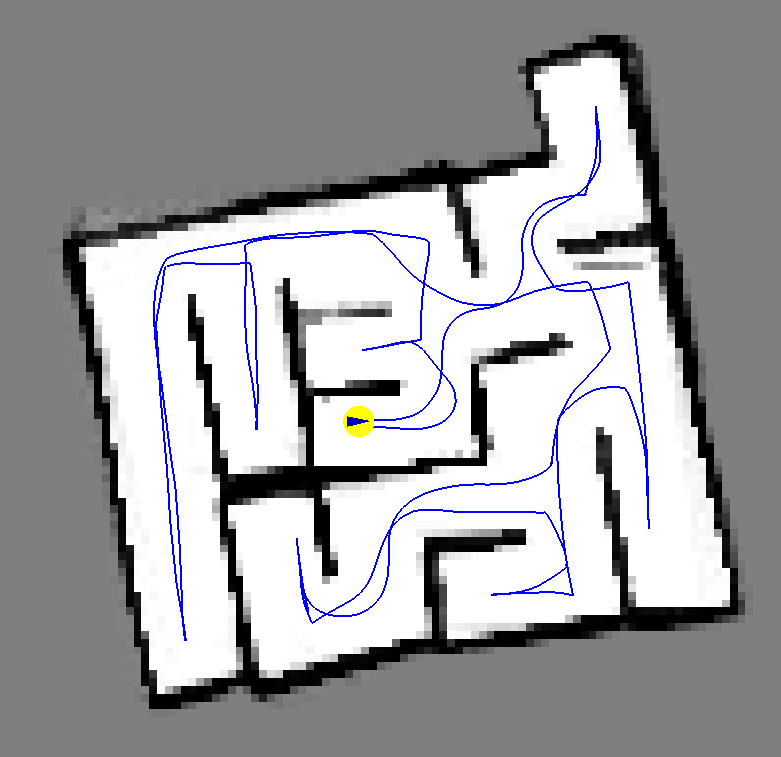
\includegraphics[width=0.3\textwidth]{Media/134.png}
\caption{Particle distribution obtained at the end of Maze Hard with Full SLAM}
\end{figure}

\section{PATH PLANNING AND EXPLORATION}

\subsection*{2.1 - Obstacle Distances} 

The obstacle distances grid code passes all the three tests in obstacle\_distance\_grid\_test, namely test for unknown distances, test for obstacle distances and test for free space distances. The code is quite optimal and there isn't anything major which tends to slow it down. The code can be made more efficient by expanding a given node to all of it 8 neighboring cells, rather than expanding it just for 4 cells.

\begin{figure}[H]
\centering
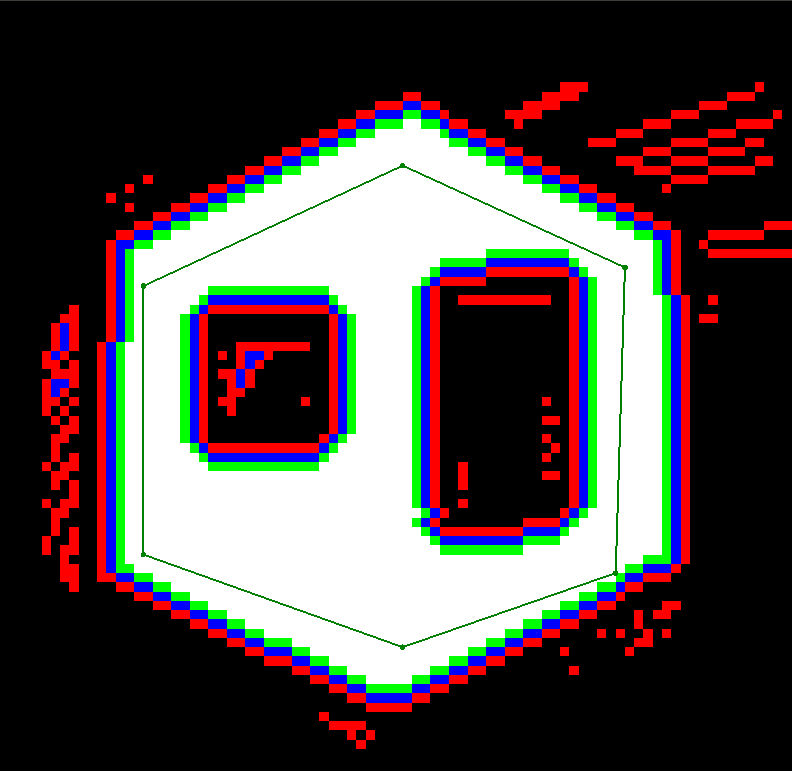
\includegraphics[width=0.3\textwidth]{Media/21.png}
\caption{Obstacle distance grid obtained at the end of Obstacle Slam with Full SLAM}
\end{figure}


\subsection*{2.2 - A* Path Planning} 

Report statistics on your path planning execution times for each of the example problems in the data/astar folder. If your algorithm is optimal and fast, great. If not please discuss possible reasons and strategies for improvement.
\\
\\
In this project A* path planning algorithm is used in conjunction with the SLAM model and the obstacle distance grid as is described in the previous sections. To test the A* star algorithm, the algorithm is executed on 6 example problems. The first test run is a map where all the cells are empty (test\_empty\_grid). The code initially fails all the test cases, because of a bug in the code, in which all the cells are initialed with -1 log odds. This situation is then mitigated by initializing the empty cell log odds by a higher number (9999). It results in an execution time for successful planning attempts of $6.81\pm1.33$ (ms). The second test run is a map of all filled grid cells, where the A* star algorithm passes the test cases with an execution time for failed planning attempts of $12.2\pm0.74$ $(\mu s)$. The next test case is a map, with a large obstacle which has a narrow passage ($<diameter_{robot}$) in between. In one of the cases the robot is instructed to move from one side of the obstacle to another, in which the robot plans a path through the constricted space and it fails, as the planned path is considered very close to the obstacles. One possible way to solve this issue is to increase the penalty of the grid cells near the obstacles. However this solution when implemented tends to take a long time to compute a path around the obstacle. The execution time for the successful planning attempts was $0.19\pm0.25$ (s). The fourth test case consists of a map which is very similar to the map in the previous test case, in which a narrow passage exists between a long obstacle, however the narrow passage in this example $\geq diameter_{robot}$. In this example the code passes all the test cases with an execution time of $0.20\pm0.27$ (s). The next test run is of a convex grid map, in which the code passes all the test cases with an execution time of $79\pm0$ $(\mu s)$. The final test case is of a maze where the robot has to plan paths between two given points. The code seems to take a long time to compute the optimal path after the first test case, hence, this test run was not fully executed. This problem can be solved by running the tests again on a system with higher computing power. 

\begin{figure}[H]
\centering
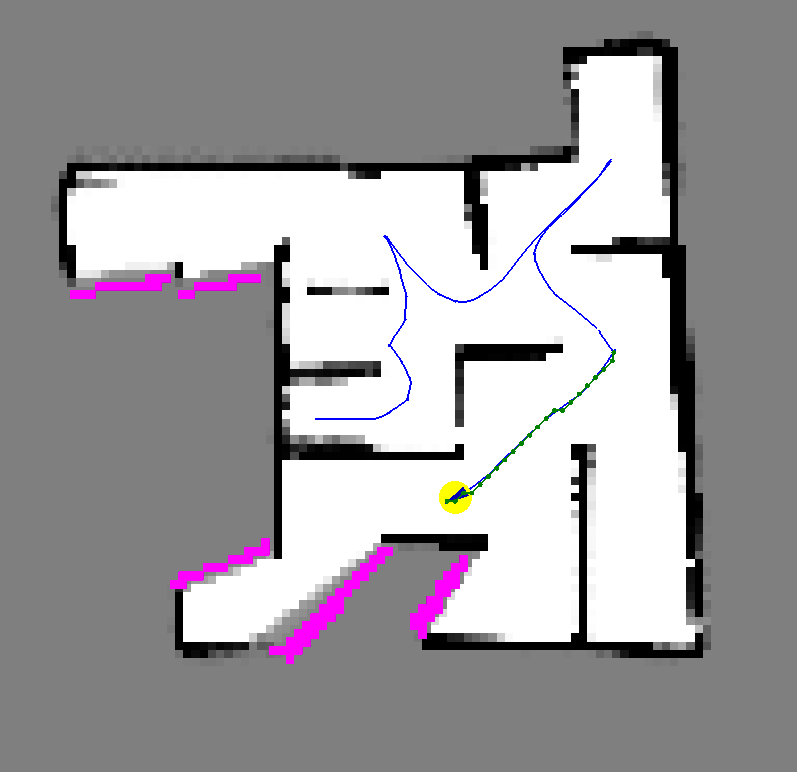
\includegraphics[width=0.3\textwidth]{Media/22.png}
\caption{Path obtained by implementing A* algorithm on Maze HiRes}
\end{figure}

\subsection*{2.3 - Map Exploration} 

Comment on your exploration performance:
 \begin{itemize}
    \item What are the factors that are preventing your exploration from being ideal?
    \item Provide your logic behind tackling frontiers (how do you go about chosing your next frontier to go to)
    \item Comments on the performance of Astar and path planning with automated exploration commands.
\end{itemize}





\ifCLASSOPTIONcaptionsoff
  \newpage
\fi

% Include your citations in the references.bib file
\nocite{*}
\bibliographystyle{IEEEtran}
\bibliography{references.bib}
\end{document}